\newpage
\chapter{Client-Server Communication}
\label{chapter06}

Communication between the Android client and the PHP based server is done over HTTP with the exchange of JSON packed messages.

\section{Hypertext Transfer Protocol}

Each time a wallpaper instance is created, a connection to the remote server must be made and a job package requested. If the connection is not possible, the data stored in the local database is used.

\begin{figure}[h]
\centering
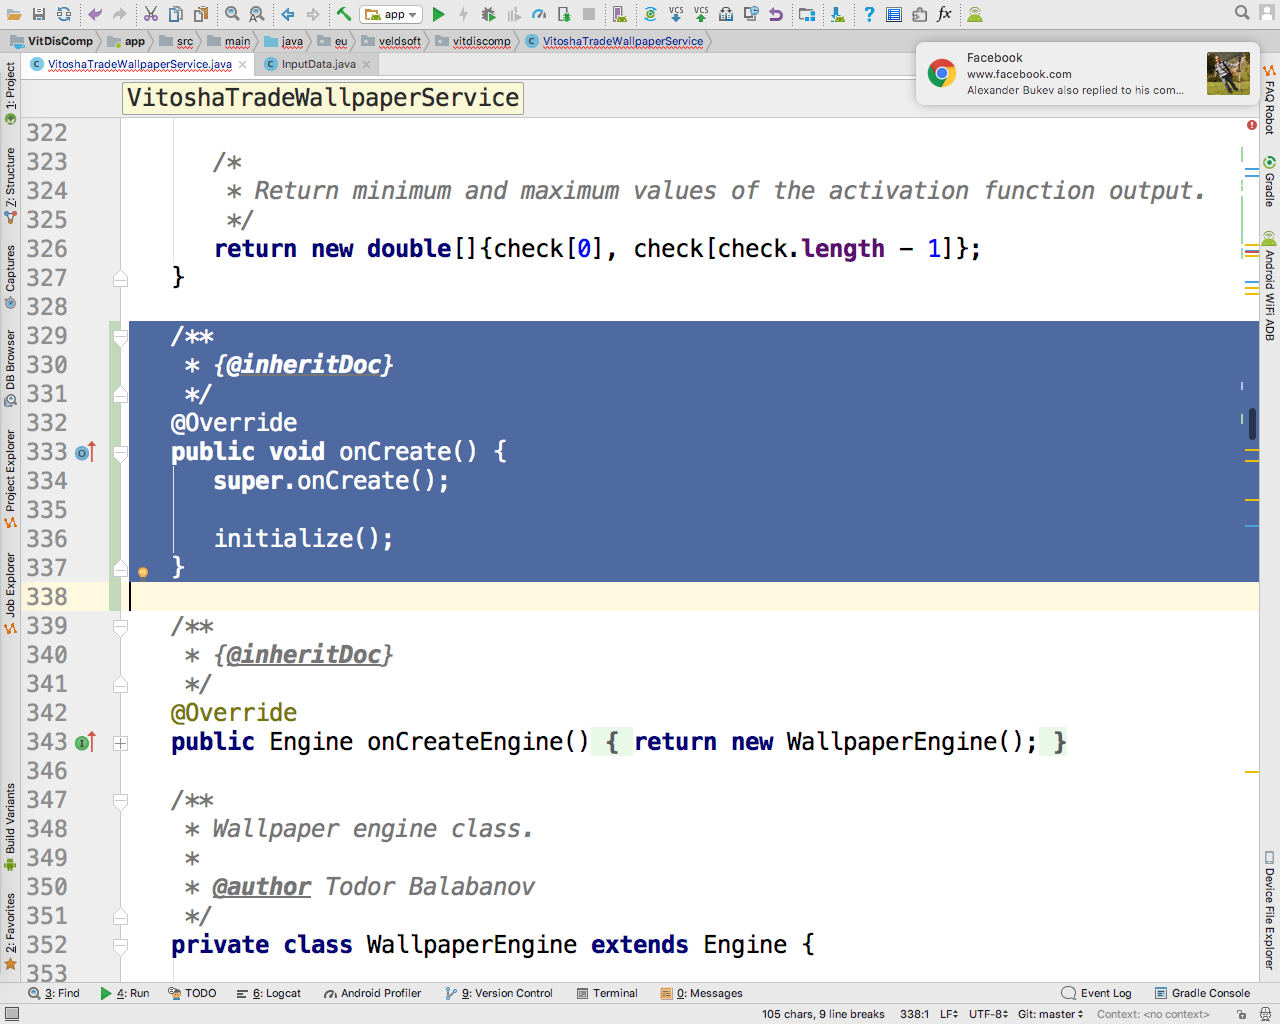
\includegraphics[height=0.45\pdfpageheight]{pic0155}
\caption{Initialization of internal variables}
\label{fig:pic0155}
\end{figure}
\FloatBarrier

Internal variables are initialized in the onCreate event (Fig. \ref{fig:pic0155}).

\begin{figure}[h]
\centering
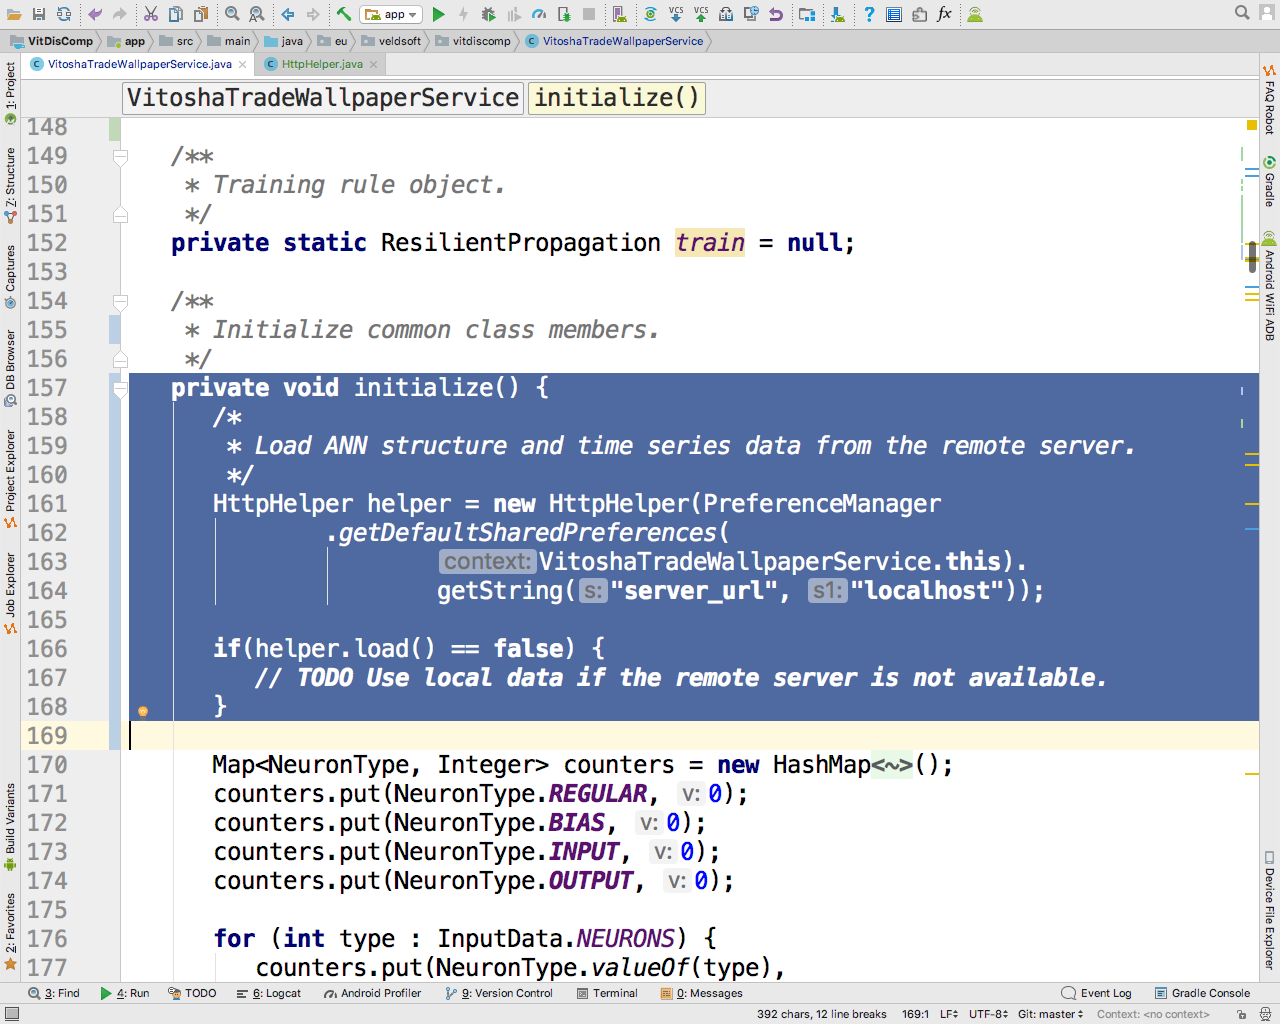
\includegraphics[height=0.45\pdfpageheight]{pic0156}
\caption{Loading data using HTTP communication}
\label{fig:pic0156}
\end{figure}
\FloatBarrier

The initialization of internal variables over HTTP is taken over by an additional created helper object, which is of a class responsible for communication (Fig. \ref{fig:pic0156}).

\begin{figure}[h]
\centering
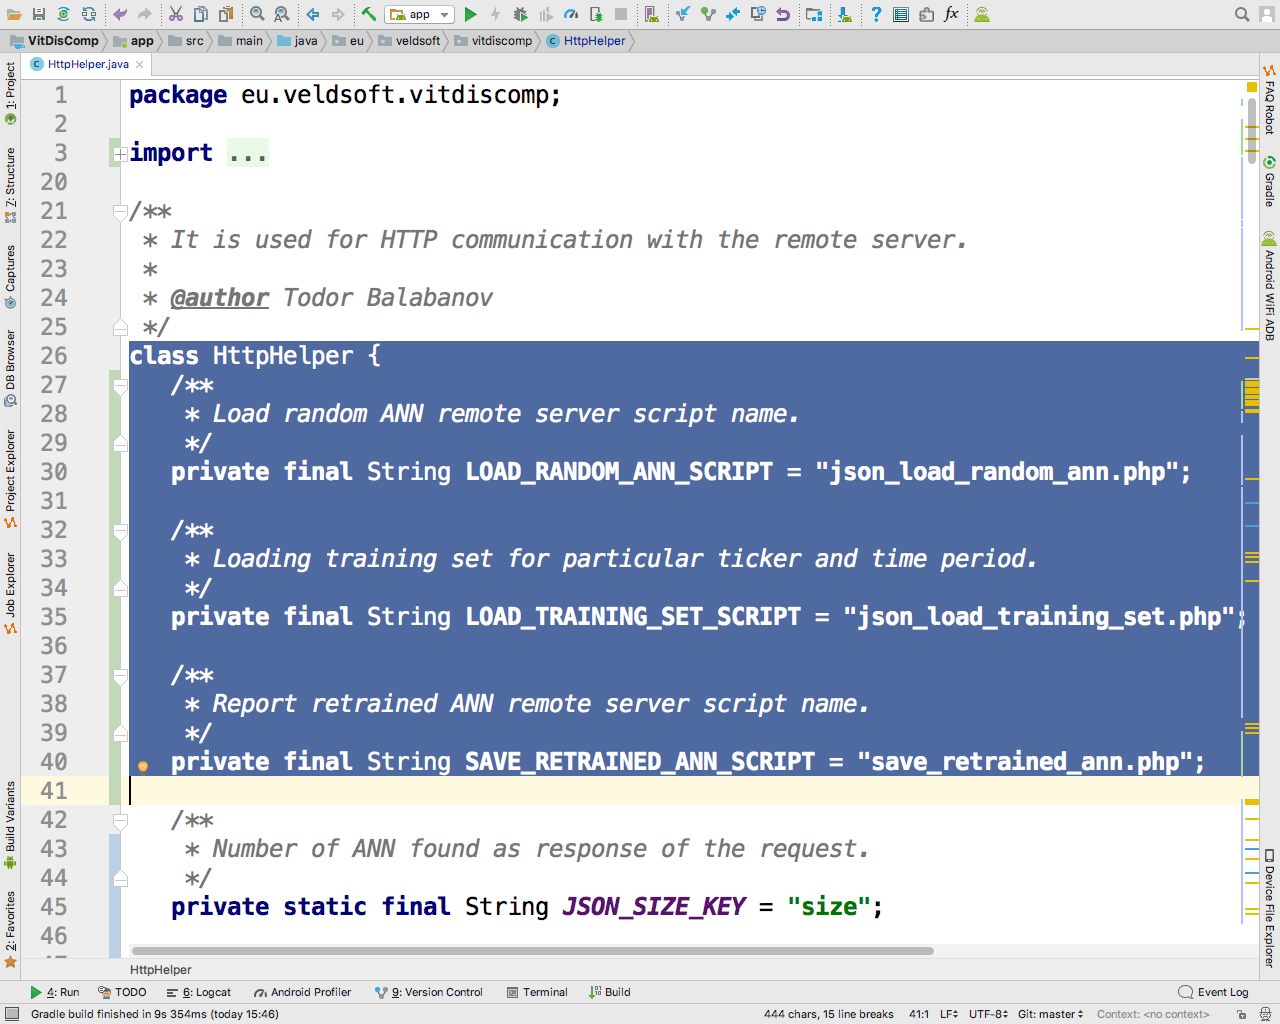
\includegraphics[height=0.45\pdfpageheight]{pic0159}
\caption{HTTP communication file}
\label{fig:pic0159}
\end{figure}
\FloatBarrier

The HTTP communication with the remote server and the parsing of the JSON messages are exported to the HttpHelper helper class (Fig. \ref{fig:pic0159}). There are various ways to set the names used for remote scripts, but one of the most basic is through named constants. Server script names are subject to change, but this is expected to be significantly less frequent than changing the URL. It is precisely for this reason that the information is parameterized in a different way.

\begin{figure}[h]
\centering
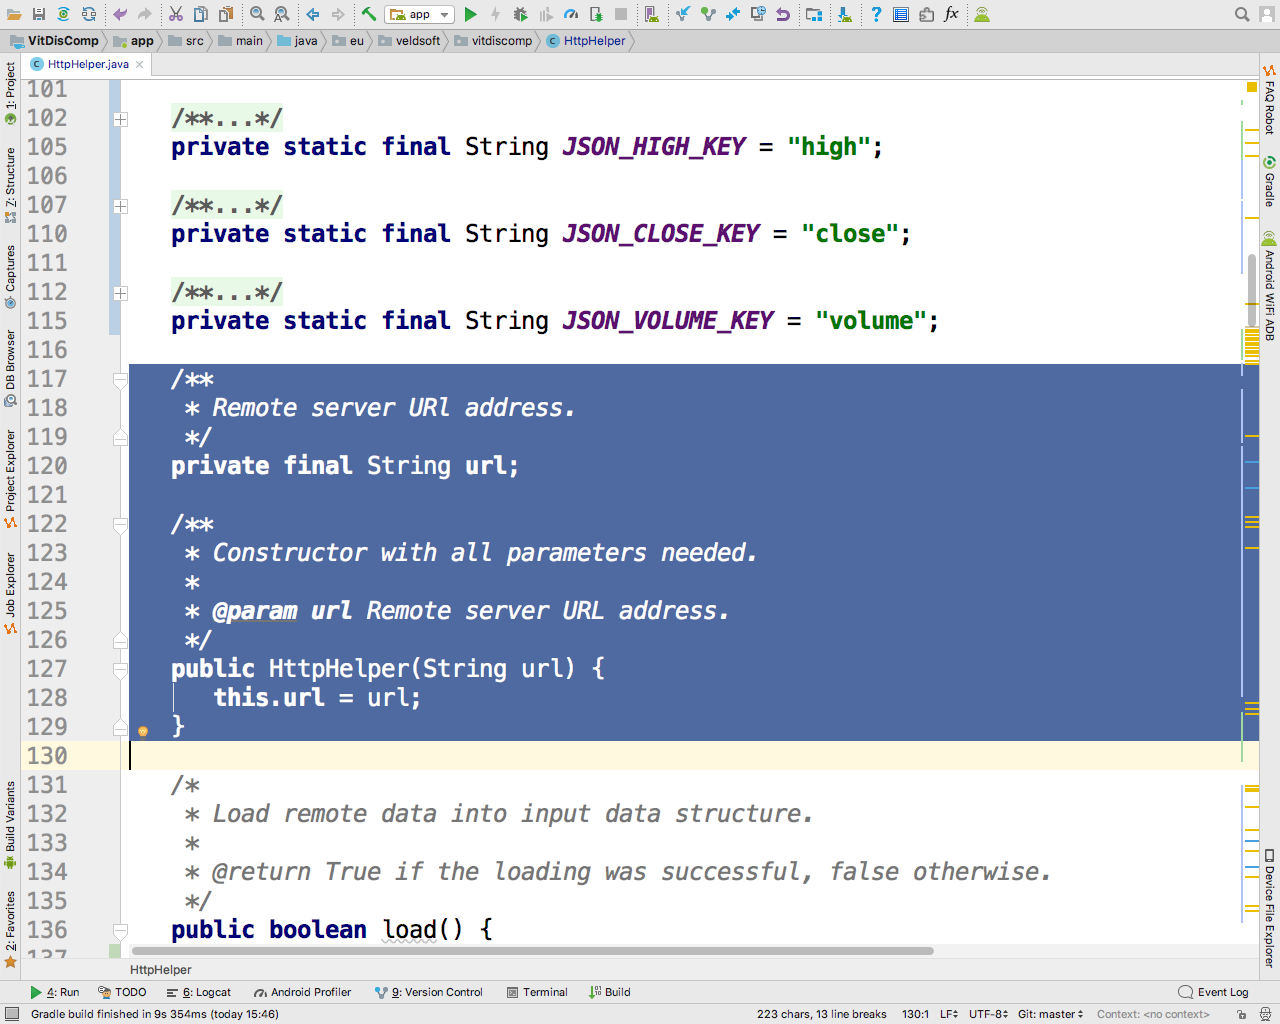
\includegraphics[height=0.45\pdfpageheight]{pic0162}
\caption{Helper class constructor}
\label{fig:pic0162}
\end{figure}
\FloatBarrier

Since the URL of the remote server is likely to change multiple times, it is wise to pass this information into the class constructor (Fig. \ref{fig:pic0162}).

\begin{figure}[h]
\centering
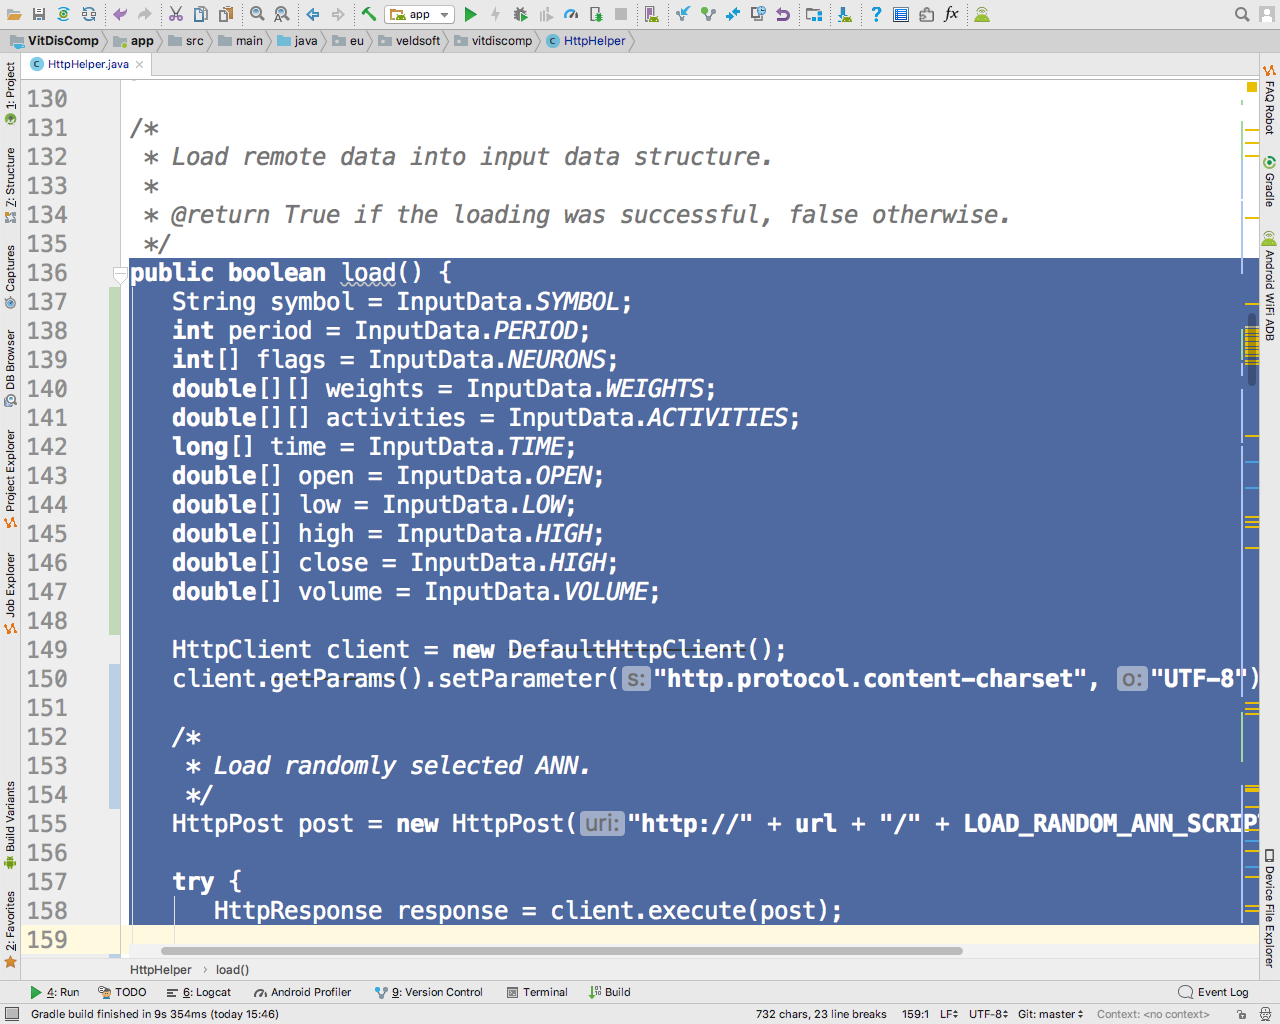
\includegraphics[height=0.45\pdfpageheight]{pic0163}
\caption{Function to load a random network selected by the server}
\label{fig:pic0163}
\end{figure}
\FloatBarrier

To spawn a random network, the designated script on the remote server is called. This is done in an auxiliary function load, which loads the information into the publicly available global structure for representing the working data (Fig. \ref{fig:pic0163}).

\begin{figure}[h]
\centering
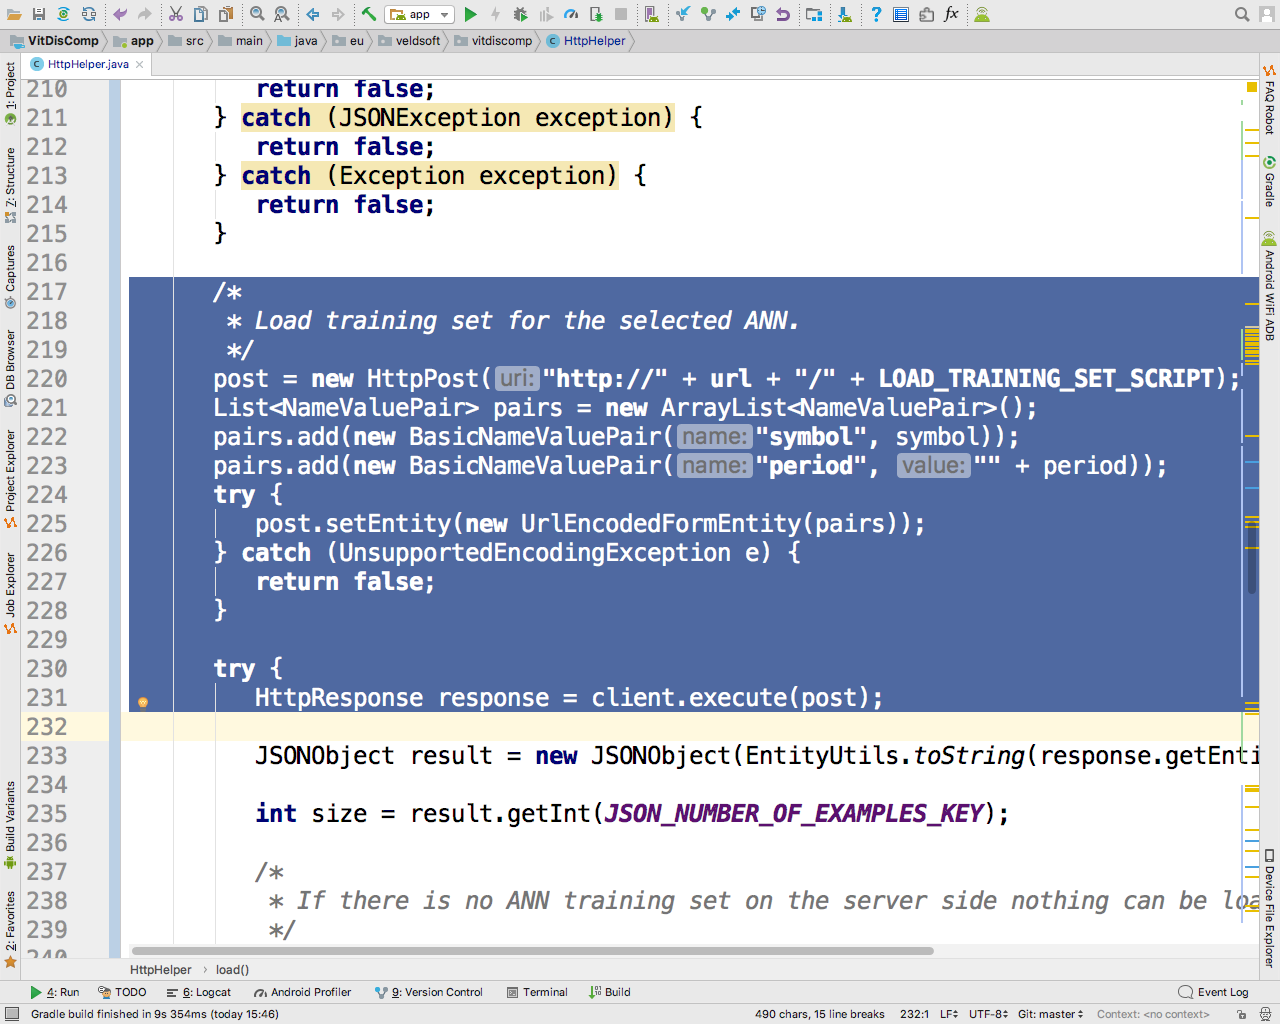
\includegraphics[height=0.45\pdfpageheight]{pic0167}
\caption{Loading training set}
\label{fig:pic0167}
\end{figure}
\FloatBarrier

After a randomly selected network is loaded, a training set suitable for the network is also loaded (Fig. \ref{fig:pic0167}). To compare the available time series, the name of the symbol pair and the period of the series are used.

\begin{figure}[h]
\centering
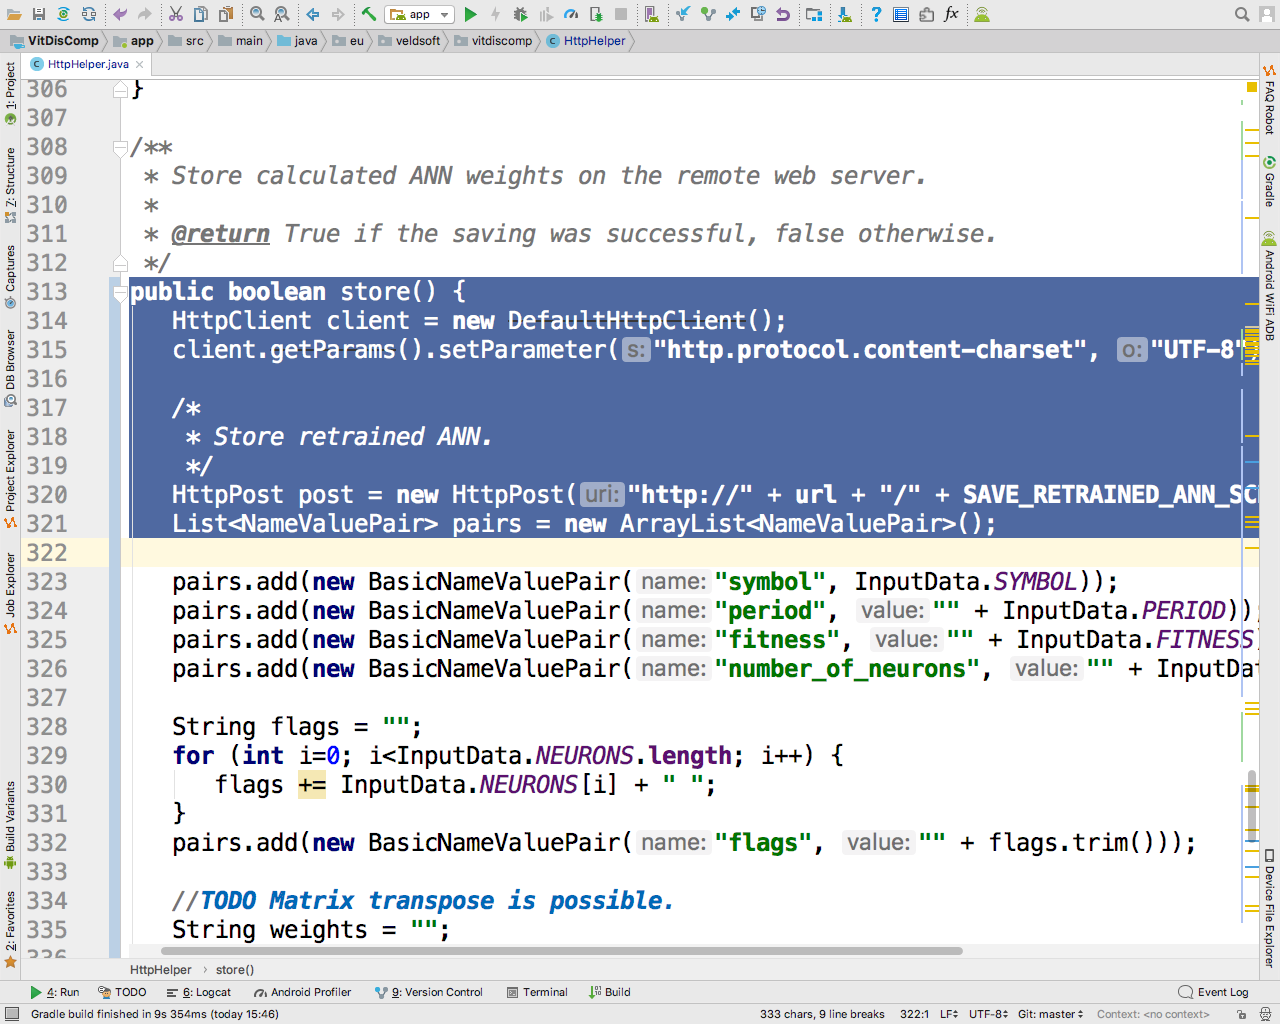
\includegraphics[height=0.45\pdfpageheight]{pic0164}
\caption{Function to save additional trained network}
\label{fig:pic0164}
\end{figure}
\FloatBarrier

In the process of storing the additionally trained network, a second helper function save is used, which aims to send, by HTTP request, the information available in the global structure with the training data (Fig. \ref{fig:pic0164}).

\begin{figure}[h]
\centering
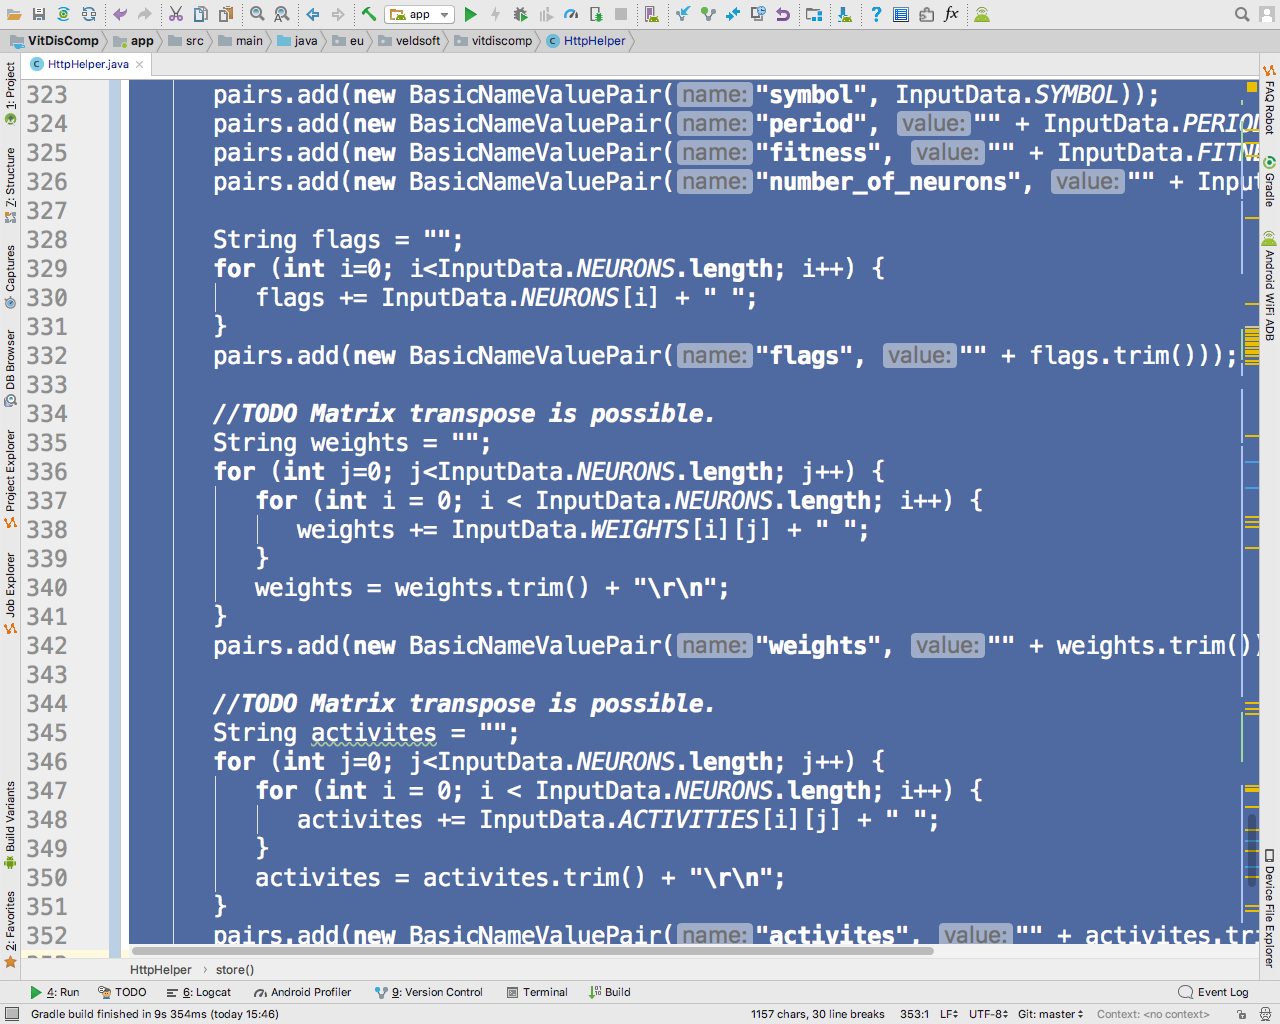
\includegraphics[height=0.45\pdfpageheight]{pic0165}
\caption{Preparing a POST request}
\label{fig:pic0165}
\end{figure}
\FloatBarrier

The data from the global structure is formed as an HTTP request of the POST type, which is related to its transformation from binary values to text (Fig. \ref{fig:pic0165}).

\begin{figure}[h]
\centering
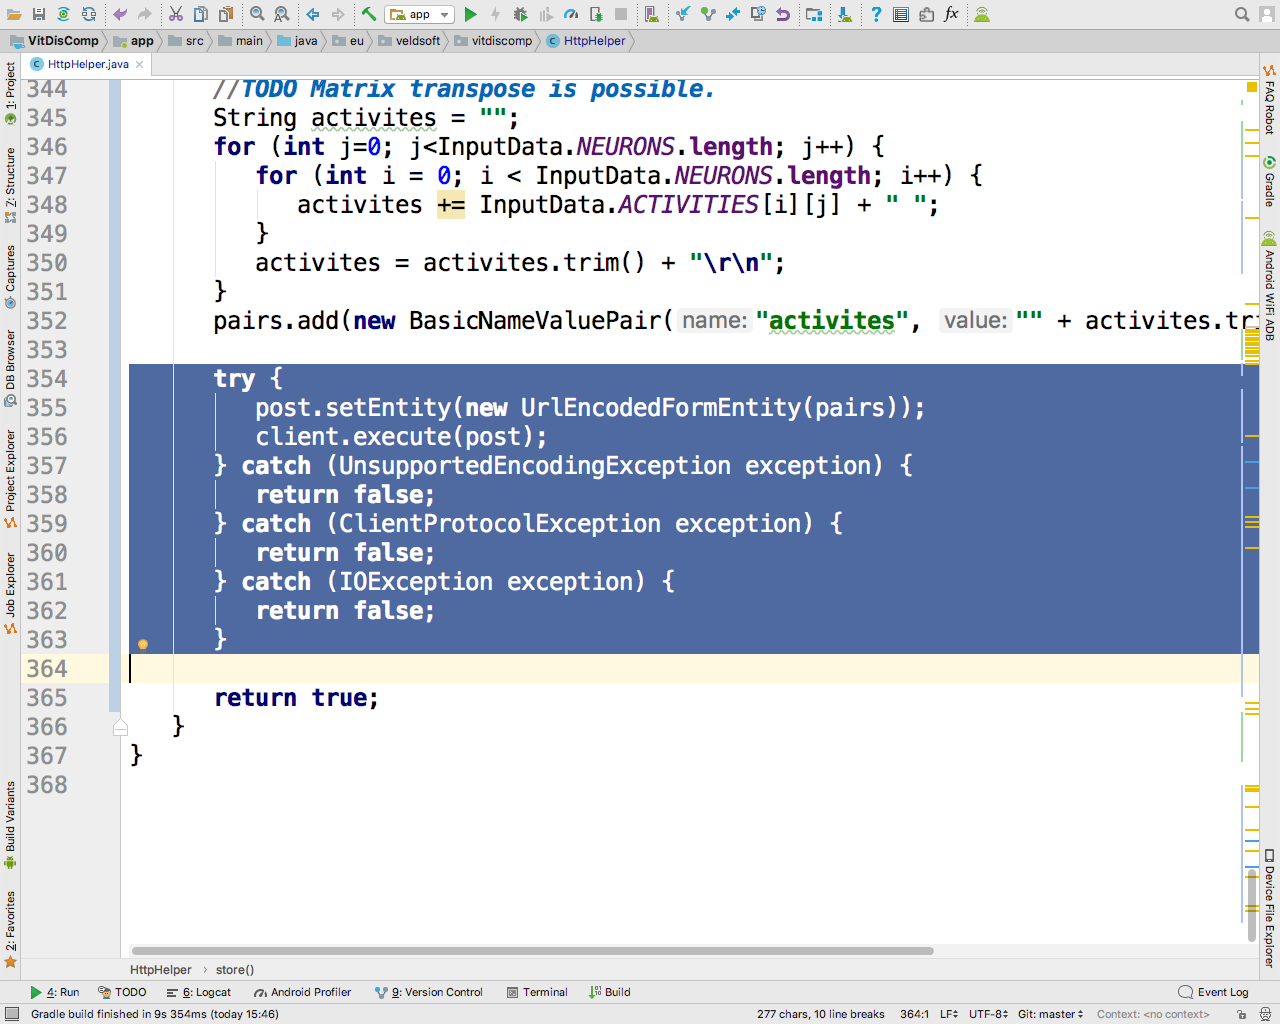
\includegraphics[height=0.45\pdfpageheight]{pic0166}
\caption{Executing the POST request}
\label{fig:pic0166}
\end{figure}
\FloatBarrier

Sending the information ends with the execution of the HTTP request (Fig. \ref{fig:pic0166}).

\section{JavaScript Object Notation}

Once received over HTTP, the JSON-packaged information is parsed and transformed from a stream of bytes into the internal structure to represent a packet for computation.

\begin{figure}[h]
\centering
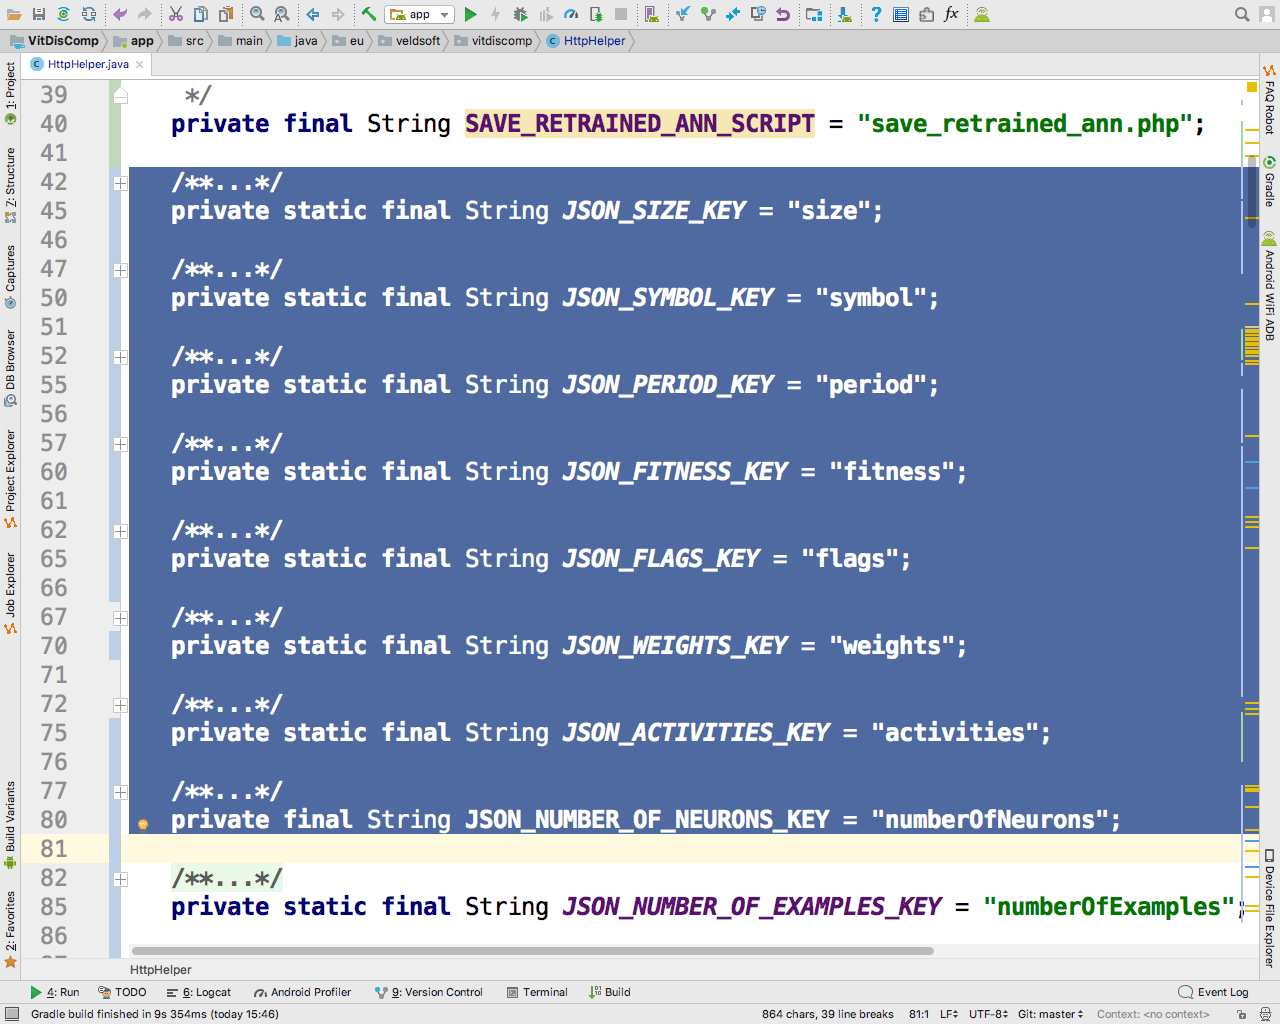
\includegraphics[height=0.45\pdfpageheight]{pic0160}
\caption{Key values to describe the network}
\label{fig:pic0160}
\end{figure}
\FloatBarrier

One of the main roles of JSON is in the construction of communication protocols, which in the present development consists of information organized hierarchically on the "key-value" principle. Since communication protocols are subject to change, it is convenient to represent key values in the form of renamed constants (Fig. \ref{fig:pic0160},\ref{fig:pic0161}).

\begin{figure}[h]
\centering
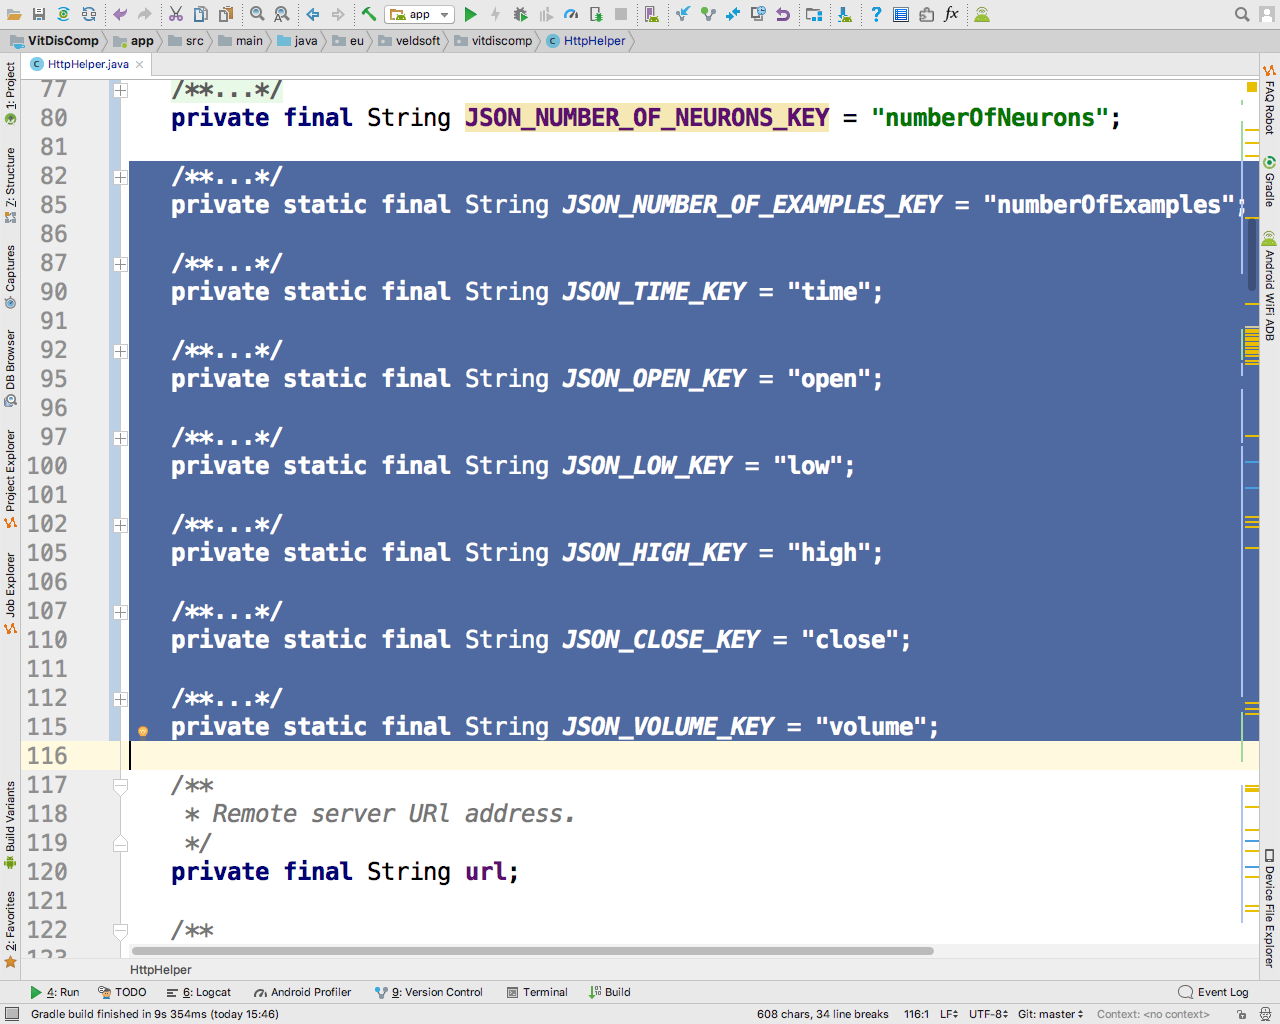
\includegraphics[height=0.45\pdfpageheight]{pic0161}
\caption{Key values to describe the training set}
\label{fig:pic0161}
\end{figure}
\FloatBarrier

When loading an artificial neural network and its training timeline from the remote server, the information is obtained with two separate HTTP requests. This requires two separate fragments to process the JSON messages.

\begin{figure}[h]
\centering
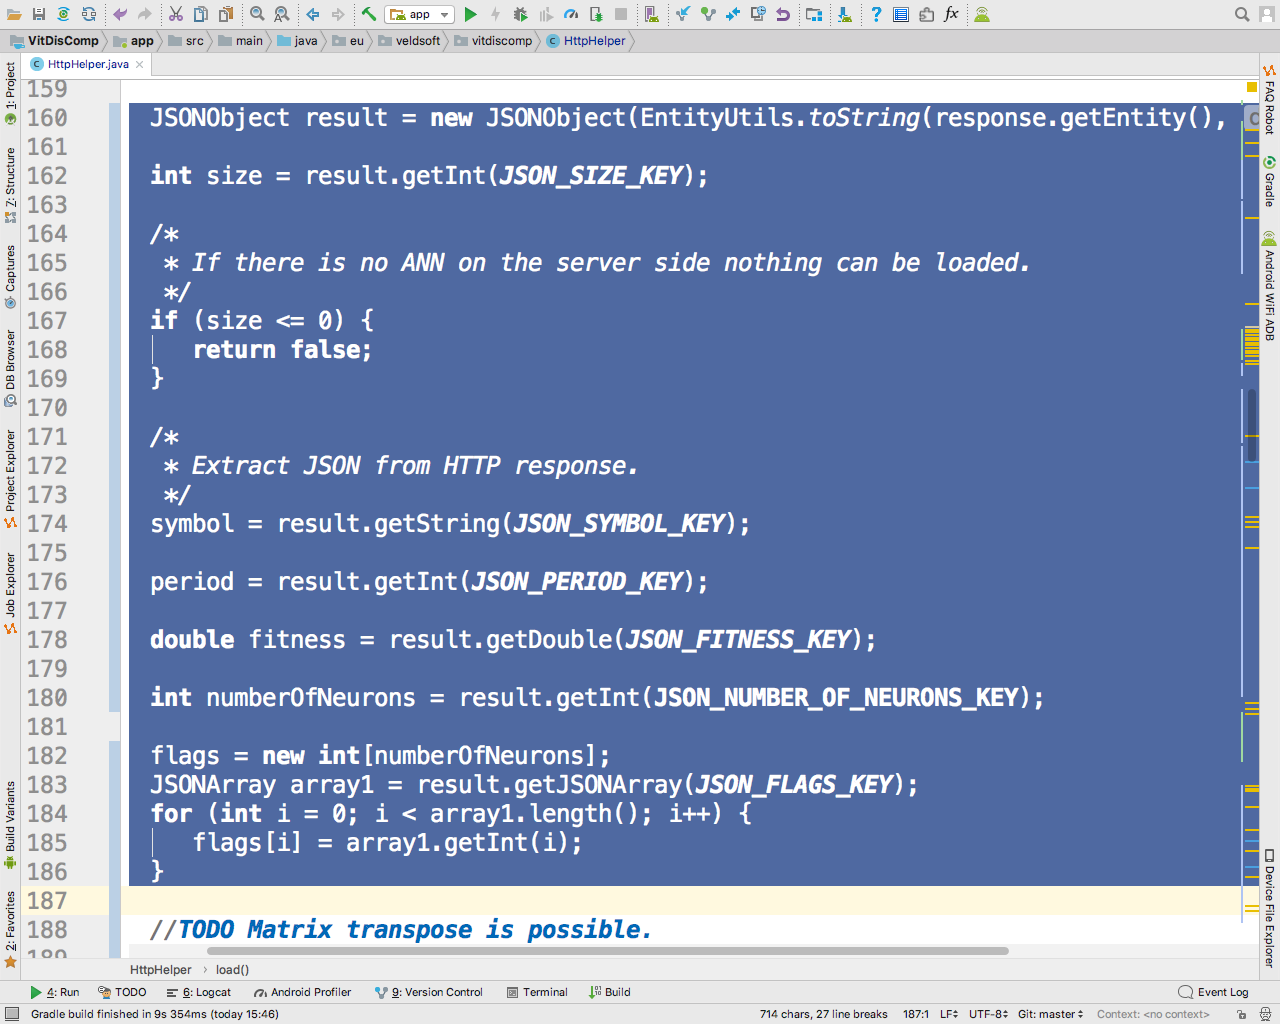
\includegraphics[height=0.45\pdfpageheight]{pic0168}
\caption{Values for time series and neurons}
\label{fig:pic0168}
\end{figure}
\FloatBarrier

The first fragment provides information about the type of time series, the period of the time series, the number of neurons in the network and their type (Fig. \ref{fig:pic0168}), values of weights and values for the strength of connections between neurons (Fig. \ref{fig:pic0169}).

\begin{figure}[h]
\centering
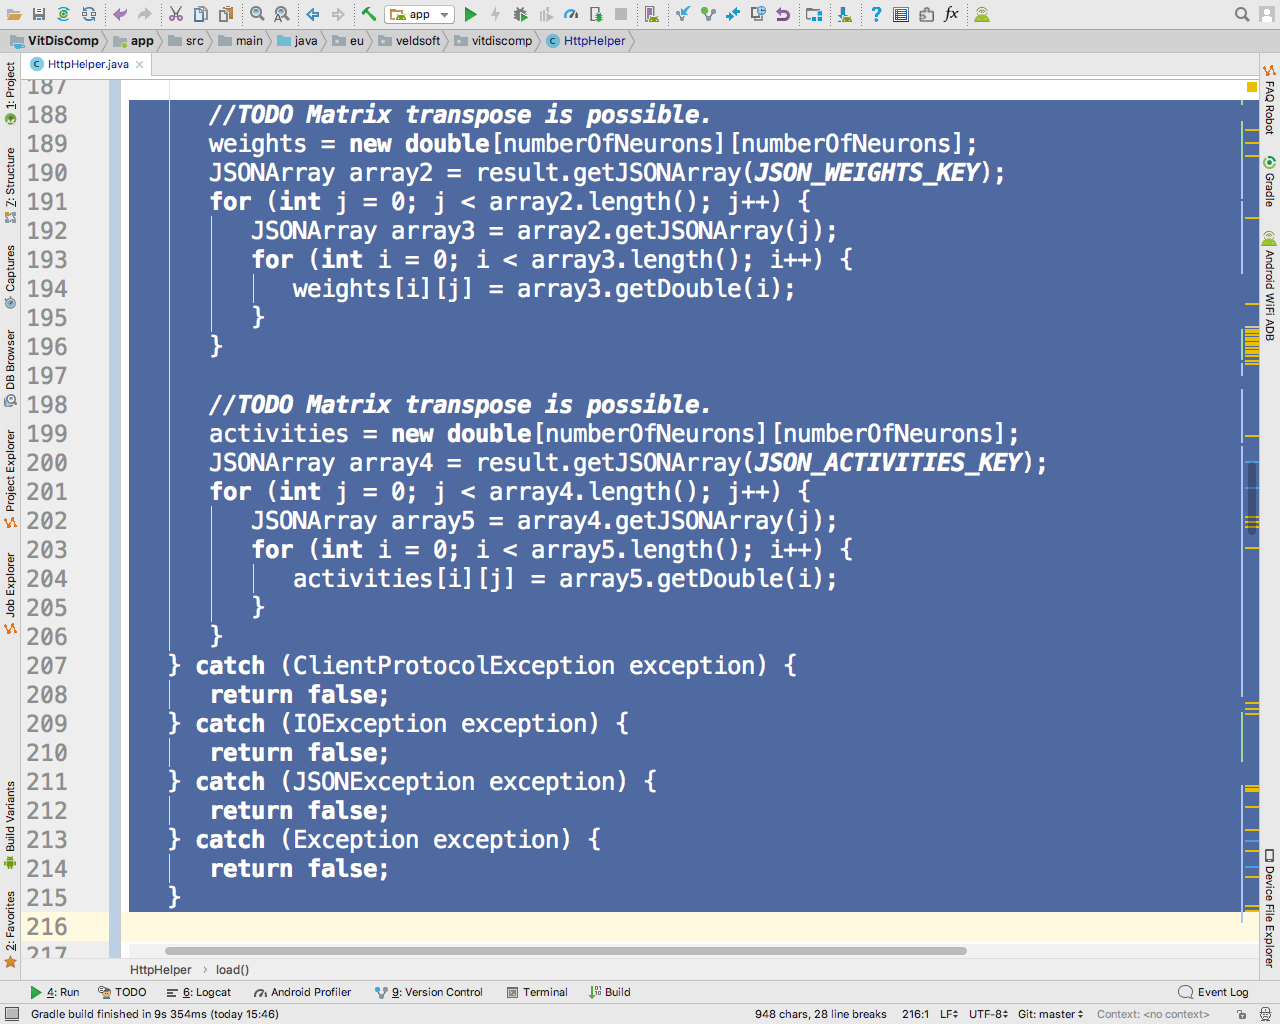
\includegraphics[height=0.45\pdfpageheight]{pic0169}
\caption{Values for link weights and strengths}
\label{fig:pic0169}
\end{figure}
\FloatBarrier

In the second fragment, information about the time series is obtained, which includes a time array, an open array, an array low (Fig. \ref{fig:pic0170}), an array high, an array close and an array for traded volume (Fig. \ ref{fig:pic0171}).

\begin{figure}[h]
\centering
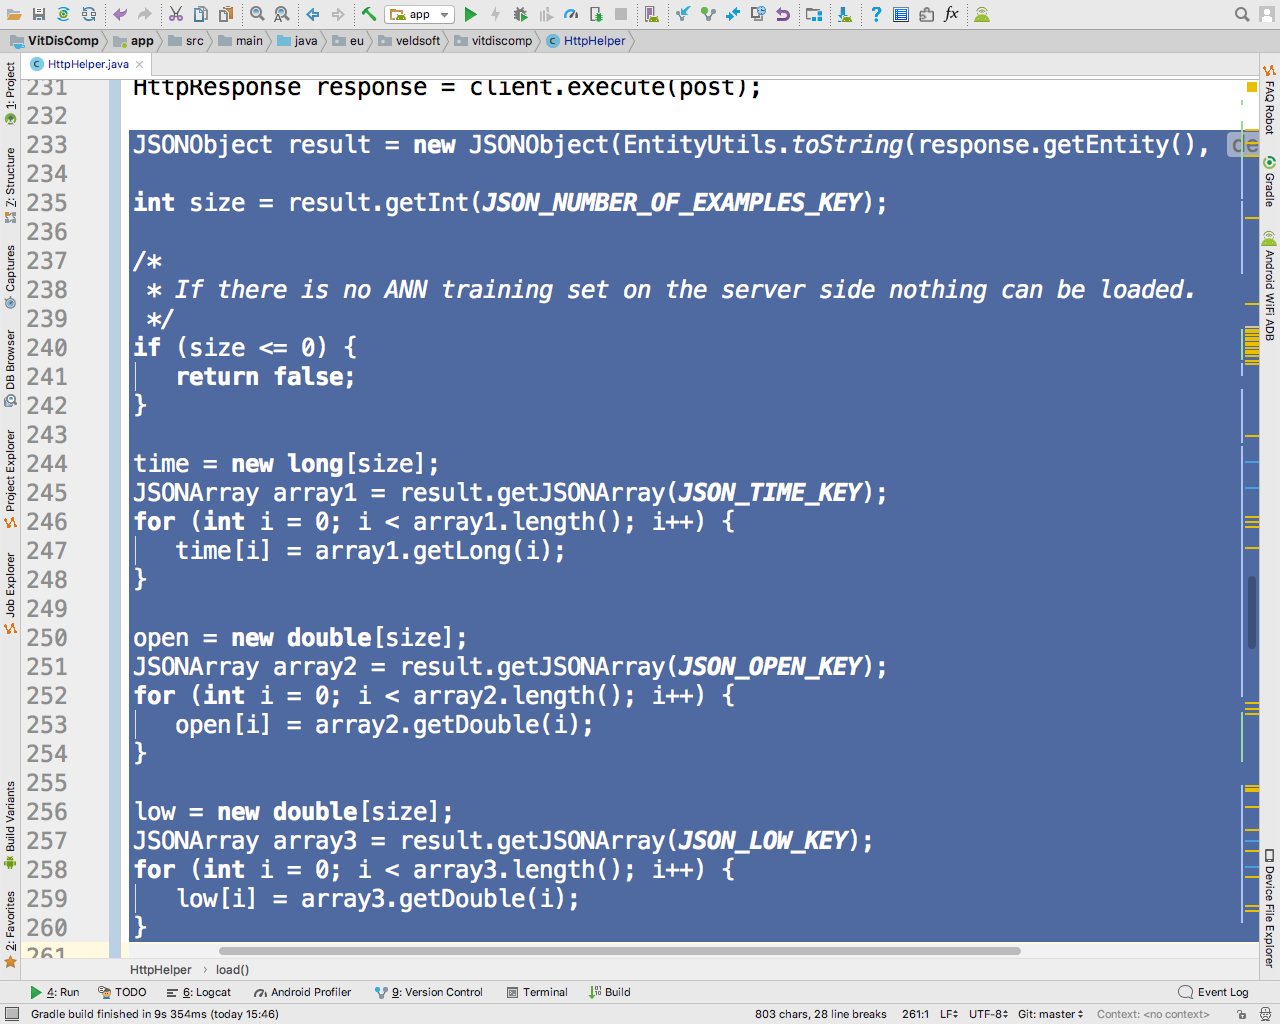
\includegraphics[height=0.45\pdfpageheight]{pic0170}
\caption{Time, Open and Lowest Hit Values}
\label{fig:pic0170}
\end{figure}
\FloatBarrier

\begin{figure}[h]
\centering
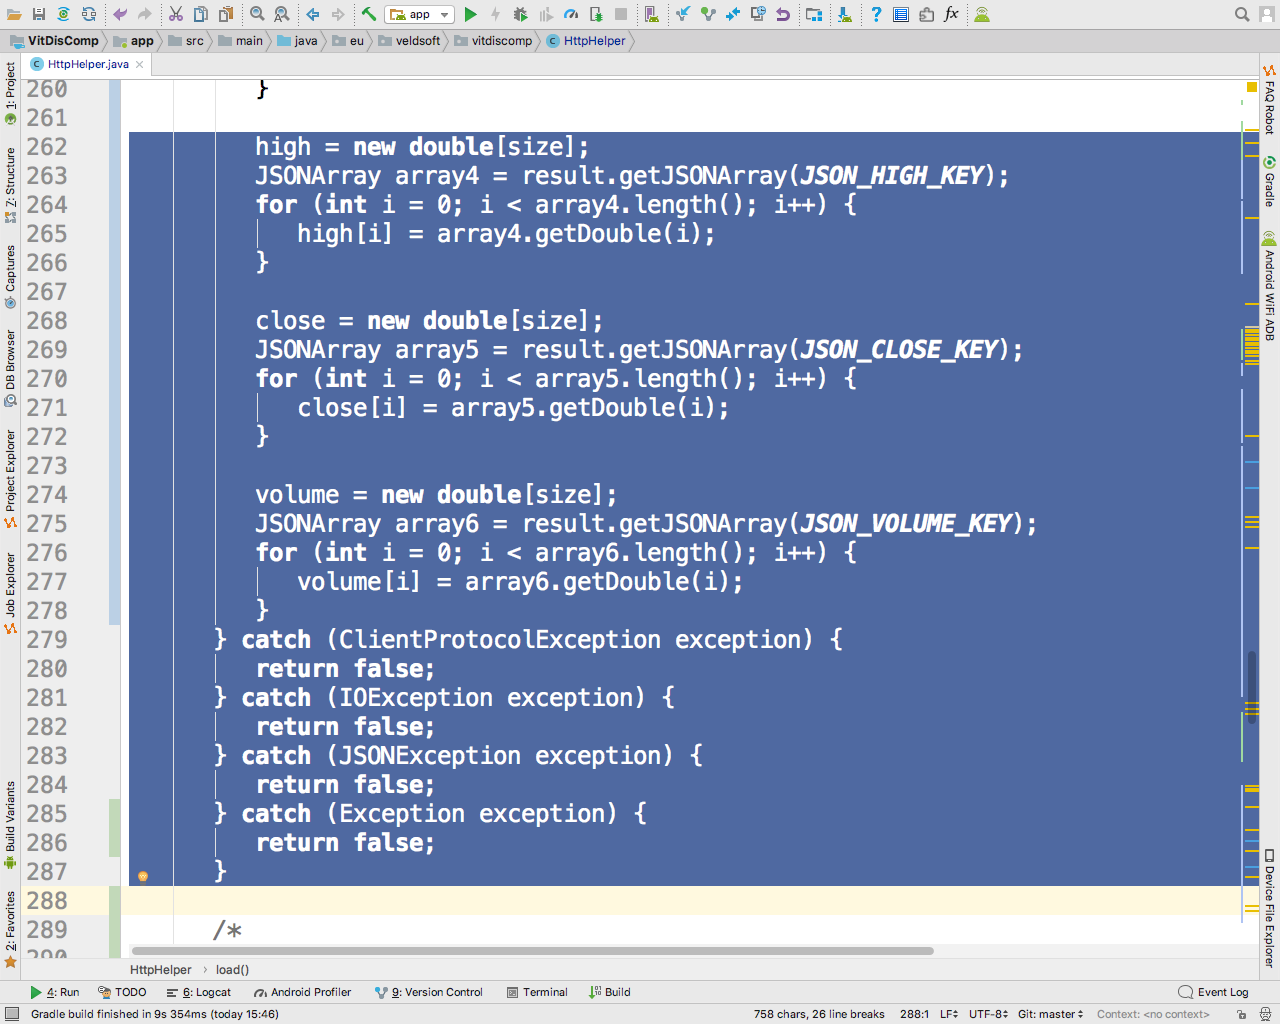
\includegraphics[height=0.45\pdfpageheight]{pic0171}
\caption{Highest Achieved Value, Close and Volume Traded}
\label{fig:pic0171}
\end{figure}
\FloatBarrier

Upon successful receipt of the information from the remote server, the data is written to the global calculation structure (Fig. \ref{fig:pic0172}).

\begin{figure}[h]
\centering
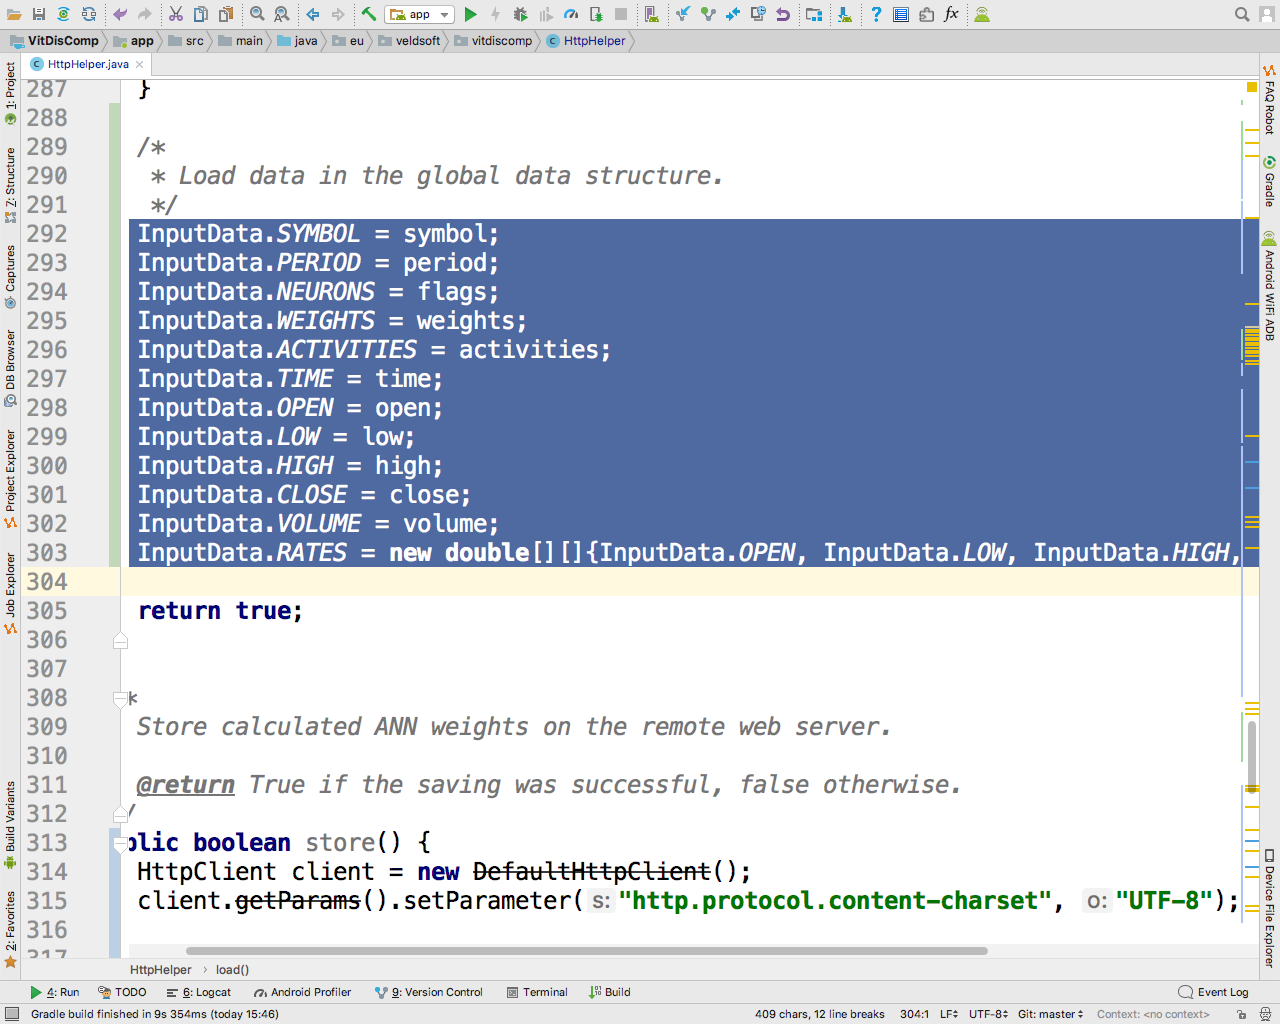
\includegraphics[height=0.45\pdfpageheight]{pic0172}
\caption{Writing the data to the global structure}
\label{fig:pic0172}
\end{figure}
\FloatBarrier
